% sample file
% http://theoval.cmp.uea.ac.uk/~nlct/latex/pdfdoc/
\documentclass{article}

\usepackage{ifthen}

\newboolean{online}
\InputIfFileExists{switch}{}{}

\ifthenelse{\boolean{online}}
{\usepackage[paperwidth=6in,paperheight=5in]{geometry}}
{\usepackage[a4paper]{geometry}}

\usepackage[nodayofweek]{datetime}
\usepackage{makeidx}
\usepackage{ifpdf}
\usepackage{graphicx}
\usepackage{pdfdoc}
\usepackage[backref=page,plainpages=false,colorlinks,bookmarks,bookmarksopen]{hyperref}
\usepackage{backrefx}

\ifthenelse{\boolean{online}}{\hypersetup{pdfpagelayout=SinglePage,pdfpagemode=None}\pagestyle{online}}{}

\ifpdf
\pdfinfo{
   /Author (Nicola Talbot)
   /Title  (Creating a PDF document using PDFLaTeX)
   /CreationDate (D:20040502195600)
   /ModDate (D:\pdfdate)
   /Subject (PDFLaTeX)
   /Keywords (PDF;LaTeX)
}
\fi

\newcommand{\appname}[1]{\texttt{#1}\indextt{#1}}
\newcommand{\Com}[1]{\texttt{\textbackslash #1}\index{#1@\textbackslash \texttt{#1}}}
\newcommand{\menu}[1]{\par\centerline{\sffamily #1}\par\noindent}
\newcommand{\indextt}[1]{\index{#1@\texttt{#1}}}
\newcommand{\sty}[1]{\texttt{#1}\index{#1 package@\texttt{#1} package}}
\newcommand{\cls}[1]{\texttt{#1}\index{#1 class file@\texttt{#1} class file}}
\newcommand{\meta}[1]{\textsf{\slshape #1}}
\newcommand{\option}[2]{\textsf{#2}\index{#1 options!#2@\textsf{#2}}}
\newcommand{\env}[1]{\textsf{#1}\index{#1 environment@\textsf{#1} environment}}

\newenvironment{definition}{\par\vspace{5pt}\noindent\ttfamily}{\par\vspace{5pt}\noindent}
\makeindex

\begin{document}
\title{Creating a PDF document using PDF\LaTeX}
\author{Nicola Talbot}
\maketitle

\tableofcontents

\ifthenelse{\boolean{online}}{\clearpage}{}
\section{Introduction}
\label{sec:intro}
This is intended as a brief introduction to using PDF\LaTeX.
For more details, I recommend that you read ``The \LaTeX\ Web Companion''~\cite{goossens1999},
and also the documentation for the \sty{hyperref} package and the documentation for PDF\TeX.

You can use PDF\LaTeX\ simply by using the command \texttt{pdflatex} instead of \texttt{latex}.  For
example if your document is called \texttt{filename.tex}, then instead of typing:
\begin{verbatim}
latex filename.tex
\end{verbatim}
you would need to type:
\begin{verbatim}
pdflatex filename.tex
\end{verbatim}
If you are using \appname{TeXnicCenter} select the output profile \verb|LaTeX => PDF|, and click
on the `Build' icon.  If you are using \appname{WinEdt}, click on the `PDF\LaTeX' icon.  If you
are using some other front-end, check the manual.

\section{Document Information}
\label{sec:pdfinfo}

When you view a PDF document in \appname{Acrobat Reader}, you can get the document information by selecting 
\menu{File$\to$Document Properties$\to$Summary}
\autoref{fig:docinfo} shows an example.

\begin{figure}[htbp]
\begin{center}
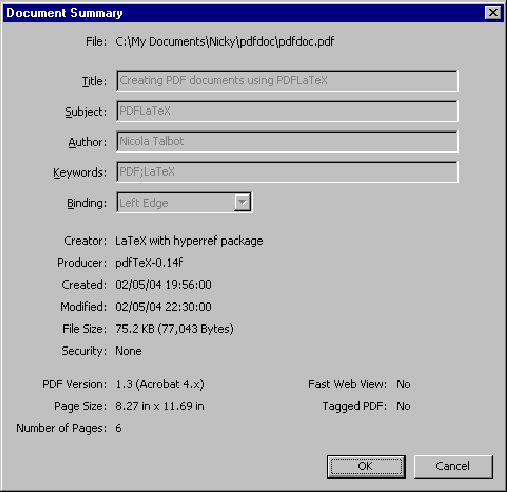
\includegraphics[scale=0.4]{docinfo}
\end{center}
\caption{Document Properties}
\label{fig:docinfo}
\end{figure}

This information can be saved to the PDF file using the command:
\begin{definition}%
\Com{pdfinfo}\{\meta{info}\}
\end{definition}%
where \meta{info} should be entered in a PDF format. For example:
\begin{verbatim}
\pdfinfo{
   /Author (Nicola Talbot)
   /Title  (Creating a PDF document using PDFLaTeX)
   /CreationDate (D:20040502195600)
   /Subject (PDFLaTeX)
   /Keywords (PDF;LaTeX)
}
\end{verbatim}
If the creation date field is omitted, the current date and time is inserted.
Note that all fields should be entered in the form:\\[5pt]
\begin{ttfamily}
/\meta{field name} (\meta{text})
\end{ttfamily}\\[5pt]
The date must be entered in the form: \texttt{D:YYYYMMDDHHmmss}.
Available fields are:\\[5pt]
\begin{tabular}{@{\ttfamily}l}
/Title\\
/Author\\
/Creator\\
/Producer\\
/CreationDate\\
/ModDate\\
/Subject\\
/Keywords
\end{tabular}\\[5pt]
The field \texttt{/ModDate} indicates the modification date, and as with
the creation date, the date should be entered in the form \texttt{D:YYYYMMDDHHmmss}.
The \href{http://theoval.cmp.uea.ac.uk/~nlct/latex/packages/index.html#datetime}{\sty{datetime}} 
package (version 2.31 and above) has the command \Com{pdfdate} which
can be used to insert the current date in the correct format.  For example:
\begin{verbatim}
\pdfinfo{
   /Author (Nicola Talbot)
   /Title  (Creating a PDF document using PDFLaTeX)
   /CreationDate (D:20040502195600)
   /ModDate (D:\pdfdate)
   /Subject (PDFLaTeX)
   /Keywords (PDF;LaTeX)
}
\end{verbatim}

Note that the command \Com{pdfinfo} is defined by PDF\LaTeX\footnote{in fact it's actually defined by PDF\TeX} but not \LaTeX, which means you'll get an error message if you try to use \LaTeX\ instead of PDF\LaTeX.  The package \sty{ifpdf}
defines the conditional \Com{ifpdf} which can be used to determine whether you are using
PDF\LaTeX\ or \LaTeX.  For example the following code:
\begin{verbatim}
This is  
\ifpdf
a PDF
\else
not a PDF
\fi
document.
\end{verbatim}
will produce the output:\\[5pt]
This is a PDF document.\\[5pt]
if PDF\LaTeX\ is used, otherwise it will produce the output:\\[5pt]
This is not a PDF document.\\[5pt]
So any commands that are specific to PDF\LaTeX\ (such as \Com{pdfinfo}) should be placed within
\Com{ifpdf} \ldots \Com{fi}. For example:
\begin{verbatim}
\ifpdf
\pdfinfo{
   /Author (Nicola Talbot)
   /Title  (Creating PDF documents using PDFLaTeX)
   /CreationDate (D:20040502195600)
   /ModDate (D:\pdfdate)
   /Subject (PDFLaTeX)
   /Keywords (PDF;LaTeX)
}
\fi
\end{verbatim}

Note that if you are using the \sty{ifthen} package, you can use\\[5pt]
\begin{ttfamily}\Com{ifthenelse}\{\Com{boolean}\{pdf\}\}\{\textrm{\ldots}\}\{\textrm{\ldots}\}\end{ttfamily}\\[5pt]
instead of\\[5pt]
\Com{ifpdf}\ldots\Com{else}\ldots\Com{fi}\\[5pt]
(but you will still need the \sty{ifpdf} package).  For example:
\begin{verbatim}
This is 
\ifthenelse{\boolean{pdf}}{a PDF}{not a PDF}
document.
\end{verbatim}
This is  
\ifthenelse{\boolean{pdf}}{a PDF}{not a PDF}
document.

\section{Including Graphics}

As with \LaTeX, the \sty{graphicx} (or \sty{graphics}) package can be used with PDF\LaTeX, however
you will no longer be able to include PostScript or Encapsulated PostScript images.  Instead, you
can use PDF images (as well as a few other formats, such as PNG).  There are applications available
for converting between various graphics formats, for example \appname{ps2pdf} and \appname{eps2pdf}.  If you want to have both
a DVI and a PDF version of your document, you would need to include the PostScript version of your image
if using \LaTeX, and the PDF version if you are using PDF\LaTeX.  Suppose you have a file called 
\texttt{shapes.ps} and you also have a PDF version called \texttt{shapes.pdf}, you could do:
\begin{verbatim}
\ifpdf
\includegraphics{shapes.pdf}
\else
\includegraphics{shapes.ps}
\fi
\end{verbatim}
however it is simpler to omit the file extension:
\begin{verbatim}
\includegraphics{shapes}
\end{verbatim}
If you are using PDF\LaTeX, the \sty{graphicx} package will assume a \texttt{.pdf} extension,
otherwise it will assume a \texttt{.ps} extension.

If you like using \sty{pstricks}, it is still possible to do so using PDF\LaTeX, however
you will need to use the \sty{pdftricks} package.  Check the \sty{pdftricks} documentation
for further information.

\section{The \texorpdfstring{\sty{hyperref}}{hyperref} Package}
\label{sec:hyperref}

We have already seen in \autoref{sec:pdfinfo} that PDF\TeX\ defines the command \Com{pdfinfo}.
There are other commands that are also defined specifically for PDF documents, however as with
all \TeX\ commands, these commands are low-level.  Fortunately, the \sty{hyperref} package provides an easy 
interface to these commands.  If you want to use the \sty{hyperref} package it is recommended that
you read the \sty{hyperref} documentation and also Chapter~2 of ``The \LaTeX\ Web Companion''~\cite{goossens1999},
as this section merely gives a brief overview of the available options.

Options\index{hyperref options} can either be specified as a comma-separated list of \meta{key}\texttt{=}\meta{value} pairs in the optional argument to the \sty{hyperref} package, e.g.
\begin{verbatim}
\usepackage[pdfpagemode=FullScreen,bookmarks=true]{hyperref}
\end{verbatim}
or as the argument to the command \Com{hypersetup}, e.g.
\begin{verbatim}
\hypersetup{pdftoolbar=true}
\end{verbatim}
If you are switching on an option, you can omit \texttt{=true}, e.g.\
\verb|\hypersetup{bookmarks}|.

One more thing to note: the \sty{hyperref} package must always be the last package to be included (unless
of course, you are using a package that modifies the behaviour of the \sty{hyperref} package, e.g.\ \sty{backrefx}).

\subsection{Cross-References and Citations}

All the cross-references and citations (using \Com{ref}, \Com{pageref} and \Com{cite}) will automatically
be converted into active links in your document when you use the \sty{hyperref} package.  The default action
is to place hyperlinks in a rectangle.  For example:
\begin{verbatim}
See section~\ref{sec:hyperref}
\end{verbatim}
will by default look like:\\[5pt]
See section~\hyperref[sec:hyperref]{\fbox{\color{black}\ref*{sec:hyperref}}}\\[5pt]
You can instead choose to omit the box and simply color the text by using the \option{hyperref}{colorlinks} option.
(e.g.\ \verb|\usepackage[colorlinks]{hyperref}|).  The above example would then look like:\\[5pt]
See section~\ref{sec:hyperref}\\[5pt]
Alternatively, the command \Com{autoref} can be used which will insert the correct context name in front
of the number.  For example:
\begin{verbatim}
See \autoref{sec:hyperref}
\end{verbatim}
will look like:\\[5pt]
See \autoref{sec:hyperref}\\[5pt]
and
\begin{verbatim}
See \autoref{fig:docinfo}
\end{verbatim}
will look like:\\[5pt]
See \autoref{fig:docinfo}

Another way of creating a hyperlink is to use the command
\begin{definition}%
\Com{hyperref}[\meta{label}]\{\meta{text}\}
\end{definition}%
For example:
\begin{verbatim}
In the \hyperref[sec:intro]{introduction} \ldots
\end{verbatim}
which would produce the following:\\[5pt]
In the \hyperref[sec:intro]{introduction} \ldots
\\[5pt]
The \sty{hyperref} package also provides starred versions of the commands \Com{ref} and \Com{pageref} which
print the relevant number, but do not create a hyperlink.  These can be used within the \Com{hyperref}
command.  For example:
\begin{verbatim}
\hyperref[sec:hyperref]{See section~\ref*{sec:hyperref}}
\end{verbatim}
would look like:\\[5pt]
\hyperref[sec:hyperref]{See section~\ref*{sec:hyperref}}

Hyperlinks to URLs can be created using the command:
\begin{definition}%
\Com{href}\{\meta{url}\}\{\meta{text}\}
\end{definition}%
For example:
\begin{verbatim}
See the 
\href{http://theoval.cmp.uea.ac.uk/~nlct/latex/csed/}{course web site} 
for further details.
\end{verbatim}
This would produce the following: 
See the 
\href{http://theoval.cmp.uea.ac.uk/~nlct/latex/csed/}{course web site} 
for further details.

Note that you don't need to worry about the tilde in the first argument to \Com{href},
nor do you have to worry about escaping the \# character:
\begin{verbatim}
\href{http://theoval.cmp.uea.ac.uk/~nlct/index.html#latex}%
{\LaTeX\ information}
\end{verbatim}
This would produce:
\href{http://theoval.cmp.uea.ac.uk/~nlct/index.html#latex}%
{\LaTeX\ information}

The \sty{hyperref} package also turns \Com{cite} commands into active links.
\begin{verbatim}
See ``The \LaTeX\ Web Companion''~\cite[Chapter~2]{goossens1999}
for further details.
\end{verbatim}
This would produce: See ``The \LaTeX\ Web Companion''~\cite[Chapter~2]{goossens1999}
for further details.  The \sty{backref} package can be used to create a set 
of back-references within the bibliography.  To implement this, use the \option{hyperref}{backref}
option to the \sty{hyperref} package.  By default this will reference the section number,
but you can change it to reference the page instead, by doing either
\begin{verbatim}
\usepackage[backref=page]{hyperref}
\end{verbatim}
or
\begin{verbatim}
\usepackage[pagebackref]{hyperref}
\end{verbatim}
There is another package \sty{backrefx} which extends the \sty{backref} package, so that
the back-references are in the form: (Cited on pages~1, 4 and 6.) instead of a simple list of numbers.
The \sty{backrefx} package should be included after the \sty{hyperref} package, e.g.:
\begin{verbatim}
\usepackage[pagebackref]{hyperref}
\usepackage{backrefx}
\end{verbatim}

Note that both the \sty{backref} and \sty{backrefx} packages assume that the bibliographic entries are
separated by a paragraph break.  This is done automatically by BiB\TeX, but it is something that you will
need to remember if you are writing the \env{thebibliography} environment by yourself.

\subsection{Table of Contents and Bookmarks}

The table of contents (produced as usual with the \Com{tableofcontents} command) will automatically 
have each entry as a hyperlink.  By default, the headings rather than the page number will be the hyperlink to the relevant chapter etc. The option \option{hyperref}{linktocpage} will swap this round.

If the option \option{hyperref}{bookmarks} is set, a set of PDF bookmarks will be created, allowing you to
navigate your way around the document.  The bookmarks can be viewed in \appname{Acrobat Reader} either by clicking on the bookmarks tab, or selecting the menu option
\menu{Window $\to$ Bookmarks}

The option \option{hyperref}{bookmarksopen} can be set if you want all the bookmark subtrees expanded,
and the option \option{hyperref}{bookmarksnumbered} can be set if you want the section numbers included in the
bookmarks.

The bookmark entries are taken from the chapter, section etc headings, but note that the text in the PDF bookmark will
not follow any \LaTeX\ formatting.

\subsubsection{An Example Heading: $a^2+b^2=c^2$}

This heading was produced with the following code:
\begin{verbatim}
\subsubsection{An Example Heading: $a^2+b^2=c^2$}
\end{verbatim}
Take a look at how this heading has appeared in the bookmarks.  \LaTeX{}ing this
document produces the following warnings:
\begin{verbatim}
Package hyperref Warning: Token not allowed in a PDFDocEncoded string,
(hyperref)                removing `math shift' on input line 319.

Package hyperref Warning: Token not allowed in a PDFDocEncoded string,
(hyperref)                removing `superscript' on input line 319.
\end{verbatim}

The command
\begin{definition}%
\Com{texorpdfstring}\{\meta{\LaTeX\ text}\}\{\meta{PDF text}\}
\end{definition}%
can be used to vary the text, depending on whether it is to be processed by \LaTeX\ or whether
it will appear in the PDF bookmark.  The above section heading could then be changed to 
\begin{verbatim}
\subsubsection{An Example Heading\texorpdfstring{: $a^2+b^2=c^2$}{}}
\end{verbatim}
In this case, the equation will be printed in the section heading within the document, but will
not appear in the bookmark.

\subsubsection{Duplicate Page Numbers}

Bookmark problems can occur when you have duplicate page numbers, for example, if you have a page~i
and a page~1. This leads to the warning:
\begin{verbatim}
! pdfTeX warning (ext4): destination with the same identifier 
(name{page.1}) has been already used, duplicate ignored
\end{verbatim} 
This can be overcome by switching off the \option{hyperref}{plainpages} option:
\begin{verbatim}
\usepackage[plainpages=false]{hyperref}
\end{verbatim}
This will change the identifiers so that they are constructed using the formatted form
of the page number instead of solely the Arabic form (e.g.\ \verb|page.i| instead of 
\verb|page.1|)  You may still find a problem arising from the title page using, say the
\cls{report} class, where although the page number does not appear, it is assigned the
page number~1, but the first page of your main matter is also page~1.  This problem can
be overcome by using a different page numbering style for the title page, that does not
occur in the rest of the document.  For example:
\begin{verbatim}
\documentclass{report}

\usepackage[plainpages=false]{hyperref}

\begin{document}
\title{A Sample Document}
\author{Me}
\pagenumbering{alph}
\maketitle
\clearpage\pagenumbering{roman}
\tableofcontents
\clearpage\pagenumbering{arabic}
\chapter{Introduction}
\end{verbatim}
In this case, switching to \texttt{alph} pagenumbering does not affect the
visual formatting as the page number does not appear on the title page, 
but it will yield unique identifiers.

\subsection{Page Layouts}

The paper size can be set by passing one of the following options to the \sty{hyperref}
package:
\begin{center}
\begin{tabular}{ll}
\bfseries Option & \bfseries Size\\
\option{hyperref}{a4paper} & $210\textrm{mm} \times 297\textrm{mm}$\\
\option{hyperref}{a5paper} & $148\textrm{mm} \times 210\textrm{mm}$\\
\option{hyperref}{b5paper} & $176\textrm{mm} \times 250\textrm{mm}$\\
\option{hyperref}{letterpaper} & $8.5\textrm{in} \times 11\textrm{in}$\\
\option{hyperref}{legalpaper} & $8.5\textrm{in} \times 14\textrm{in}$\\
\option{hyperref}{executivepaper} & $7.25\textrm{in} \times 10.5\textrm{in}$
\end{tabular}
\end{center}
It is also possible to set the following options which can be used to change the display options
(see ``The \LaTeX\ Web Companion''~\cite{goossens1999} for a complete list):
\begin{center}
\begin{tabular}{lp{0.6\textwidth}}
\bfseries Option & \bfseries Action\\
\option{hyperref}{pdfcenterwindow} & Position window displaying document in centre of the screen\\
\option{hyperref}{pdffitwindow} & Resizes window displaying document  to fit the size of the first displayed page of the document.\\
\option{hyperref}{pdftoolbar} & Sets the toolbar to be visible (\texttt{=true}) or not visible (\texttt{=false})\\
\option{hyperref}{pdfmenubar} & Sets the menu bar to be visible (\texttt{=true}) or not visible (\texttt{=false})\\
\option{hyperref}{pdfpagelayout} & Sets the page layout when the document is opened.  This can take the 
values: \texttt{SinglePage}, \texttt{OneColumn}, \texttt{TwoColumnLeft}, \texttt{TwoColumnRight}
\end{tabular}
\end{center}

\subsection{Acrobat Menu Command}

The command
\begin{definition}%
\Com{Acrobatmenu}\{\meta{menuitem}\}\{\meta{text}\}
\end{definition}%
can be used to access the relevent Acrobat menu item, where \meta{menuitem} is the Acrobat menu option name
and \meta{text} is the link text.  For example:
\begin{verbatim}
\Acrobatmenu{GeneralInfo}{Document Summary}
\end{verbatim}
will produce:
\Acrobatmenu{GeneralInfo}{Document Summary}.  Note that \meta{text} doesn't have to simply be text, it can be
any \LaTeX\ code, which means you could use a picture instead.  A full list of menu options is given in ``The \LaTeX\
Web Companion''~\cite{goossens1999}, but the most commonly used ones are: \texttt{PrevPage}, \texttt{NextPage},
\texttt{FirstPage}, \texttt{LastPage}, \texttt{GoBack}, \texttt{GoForward} and \texttt{Quit}.  It is therefore
possible to incorporate your own navigation panel within your document by defining a new page style that includes
\Com{Acrobatmenu} commands.

For example, this document defines a new page style called \texttt{online}%
\ifonline \else, which is used for the on-line version,\fi\
and is defined as follows:
\begin{verbatim}
\newcommand\ps@online{
\renewcommand{\@oddhead}{}
\renewcommand{\@evenhead}{}
\renewcommand{\@oddfoot}{\hfill
   \Acrobatmenu{PrevPage}{Previous}
   \Acrobatmenu{NextPage}{Next}
   \Acrobatmenu{FirstPage}{First}
   \Acrobatmenu{LastPage}{Last}
   \Acrobatmenu{GoBack}{Back}
   \Acrobatmenu{GoForward}{Forward}
   \hyperref[sec:index]{Index}\hfill\thepage}
\renewcommand{\@evenfoot}{\@oddfoot}}
\end{verbatim}
As can be seen the headers are blank, and the footer contains the \Com{Acrobatmenu} commands.
It also uses the \Com{hyperref} command to provide a link to the index, and the \Com{hfill}
commands neatly centre the text, with the page number pushed to the far right.  
The \env{theindex} environment was also redefined so that
it incorporated the \verb|\label{sec:index}| command.  This was necessary because \Com{printindex}
starts a new page, so placing the label before this command would link to the page before
the index, and placing the label after \Com{printindex} would link to the end of the index.

\section{Strange Errors or Unexpected Ouput}

This section lists some errors or unexpected results that you may encounter using PDF\LaTeX.

\begin{itemize}
\item The links in my index and backref citations go to the absolute page rather than the \LaTeX\ page
even though I'm using the \texttt{plainpages=false} option.

There are some packages that seem to interfere with the commands that generate these links.  I've noticed
that using the \sty{subfigure} package can cause this problem.

\item I get the error
\begin{verbatim}
pdfTeX error (ext4): link annotations can't be nested.
\grf@@shipout ->\grf@org@shipout \box \@cclv 
                                             \relax
\end{verbatim}
but I don't have any nested annotations.

This error can be caused by a page break occuring in the middle of a link.  For example, suppose
you have the following:
\begin{verbatim}
\hyperref[sec:optional]{optional arguments}
\end{verbatim}
If a page break occurs between the words ``optional'' and ``arguments'', a shipout command will
occur whilst a link is still being created, which will cause the error.  To get around this, you
can split the link up into two links:
\begin{verbatim}
\hyperref[sec:optional]{optional}
\hyperref[sec:optional]{arguments}
\end{verbatim}

\item Some of my fonts haven't come out.

PDF\LaTeX\ can't handle PostScript fonts, so check to see if you have included any package that use
PostScript fonts (such as \sty{pifont}).
\end{itemize}

\bibliographystyle{plain}
\bibliography{pdfdoc}
\addcontentsline{toc}{section}{\refname}
\printindex

\end{document}

